
\begin{frame}[ctb!]
  \frametitle{FCS History}

  \begin{columns}[t]

    \column{.33\textwidth}
    \begin{block}{Spreadsheets}
      \begin{itemize}
        \item very inextensible
        \item basic output
        \item little to no decision making
      \end{itemize}
    \end{block}

    \pause

    \column{.33\textwidth}
    \begin{block}{Simulation Dynamics}
      \begin{itemize}
        \item limited extensibility
        \item aggregate mass flows
        \item limited \textit{in situ} decision making
        \item fleet based
      \end{itemize}
    \end{block}

    \pause

    \column{.33\textwidth}
    \begin{block}{Next Generation FCS}
      \begin{itemize}
        \item extensible
        \item \textit{in situ} decision making
        \item isotopic-based dynamics
        \item facility-level effects
        \item region-level effects
      \end{itemize}
    \end{block}

  \end{columns}
  
\end{frame}

\begin{frame}[ctb!]
  \frametitle{Issues with Current SD Implementations}
  
  \begin{itemize}
    \item fleet-based models lack facility-level detail (e.g., facility
      disruptions, facility location, transportation, etc.)
    \item aggregate mass flows lack isotopic-level detail
    \item static facility (fleet) connections
    \item equation-based model limits simulation extensibility
    \item little-to-no recycled fuel matching fidelity
  \end{itemize}

\end{frame}

\begin{frame}[ctb!]
  \frametitle{Basic \Cyclus Approach}

  \begin{itemize}
    \item treat facilities individually
    \item facilities discretely transact materials
    \item materials are defined by both an isotopic \textit{quality} and
      quantity
    \item designed with extensibility in mind
  \end{itemize}

\end{frame}

\begin{frame}[ctb!]
  \frametitle{Making \Cyclus Extensible}
  
  Facilities, materials (i.e., commodities) are treated generally in \Cyclus.

  \begin{figure}
    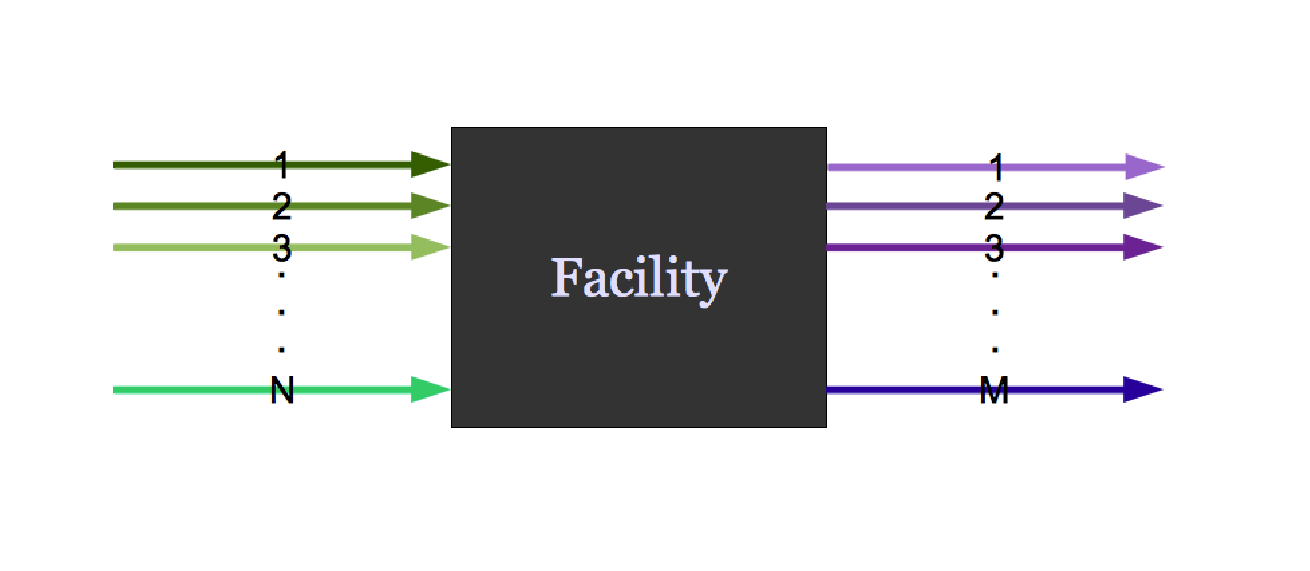
\includegraphics[height=4cm]{./images/facs.eps}
    \caption{Facilities as black boxes. \cite{cyclus2012}.}
    \label{fig:facs}  
  \end{figure}

\end{frame}

\begin{frame}[ctb!]
  \frametitle{Issues with Current Recycled Fuel Matching}
  
  Current implementations of the modeling of recycled fuel fabrication
  \begin{itemize}
    \item lack rigor
    \item don't account for element-isotope issues present at this interface
  \end{itemize}
  
  \vspace{0.2cm}

  VISION models the process by:
  \begin{itemize}
    \item placing separated isotopes in ``bins''
    \item declaring ``control isotopes''
    \item removing the correct control isotopes fraction from the bin
  \end{itemize}
  
\end{frame}

\begin{frame}[ctb!]
  \frametitle{Issues with Current Recycled Fuel Matching}

  COSI's uses the ``Equivalence Model'', adapted from a method introduced in
  1963 by Baker and Ross\cite{baker_comparison_1963}.
  
  \vspace{0.2cm}

  Method and implementation outline:
  \begin{itemize}
    \item used for recycled fuel recipes
    \item assumes ``ideal'' recipe of $^{239}$Pu and $^{238}$U
    \item determines a recipe given ``bins'' of fissile and fertile material
  \end{itemize}
\end{frame}

\begin{frame}[ctb!]
  \frametitle{Issues with Current Recycled Fuel Matching}

  In such a model, the following are defined:
  \begin{itemize}
    \item a quantity of fuel
    \item a target Pu-239 enrichment, $E_0$
    \item a ``bin'' of fertile isotopes
    \item a ``bin'' of fissile isotopes
  \end{itemize}

  And its output is:
  \begin{itemize}
    \item a weight fraction, $E$, to extract from the fissile isotopes
    \item a weight fraction, $1-E$, to extract from the fertile isotopes
  \end{itemize}
\end{frame}

\begin{frame}[ctb!]
  \frametitle{Issues with Current Recycled Fuel Matching}
  
  An isotopic ``worth'' is defined for each isotope, $i$, as:
  \begin{equation}
    w_i = \frac{x_i - x_{^{238}U}}
    {x_{^{239}Pu} - x_{^{238}U}}.
  \end{equation}

  with $x_i$ defined as:
  
  \begin{equation}
    x_i = \nu_{i} \sigma_{f,i} - \sigma_{a,i}
  \end{equation}

  with physical parameters:
  \begin{itemize}
    \item $\nu_{i}$ - average number of neutrons resulting from fission
    \item $\sigma_{f,i}$ - microscopic fission cross section
    \item $\sigma_{a,i}$ - microscopic absorption cross section
  \end{itemize}
\end{frame}

\begin{frame}[ctb!]
  \frametitle{Issues with Current Recycled Fuel Matching} 
  
  With isotopic weight fractions, $\xi_i$, the fissile fraction, $E$, is given
  by:
  \begin{equation}
    E = \frac{E_0 - \sum_{i \in I_{Fe}} \xi_i w_i}
    {\sum_{i \in I_{Fi}} \xi_i w_i - \sum_{i \in I_{Fe}} \xi_i w_i}.
  \end{equation}

  \begin{figure}
    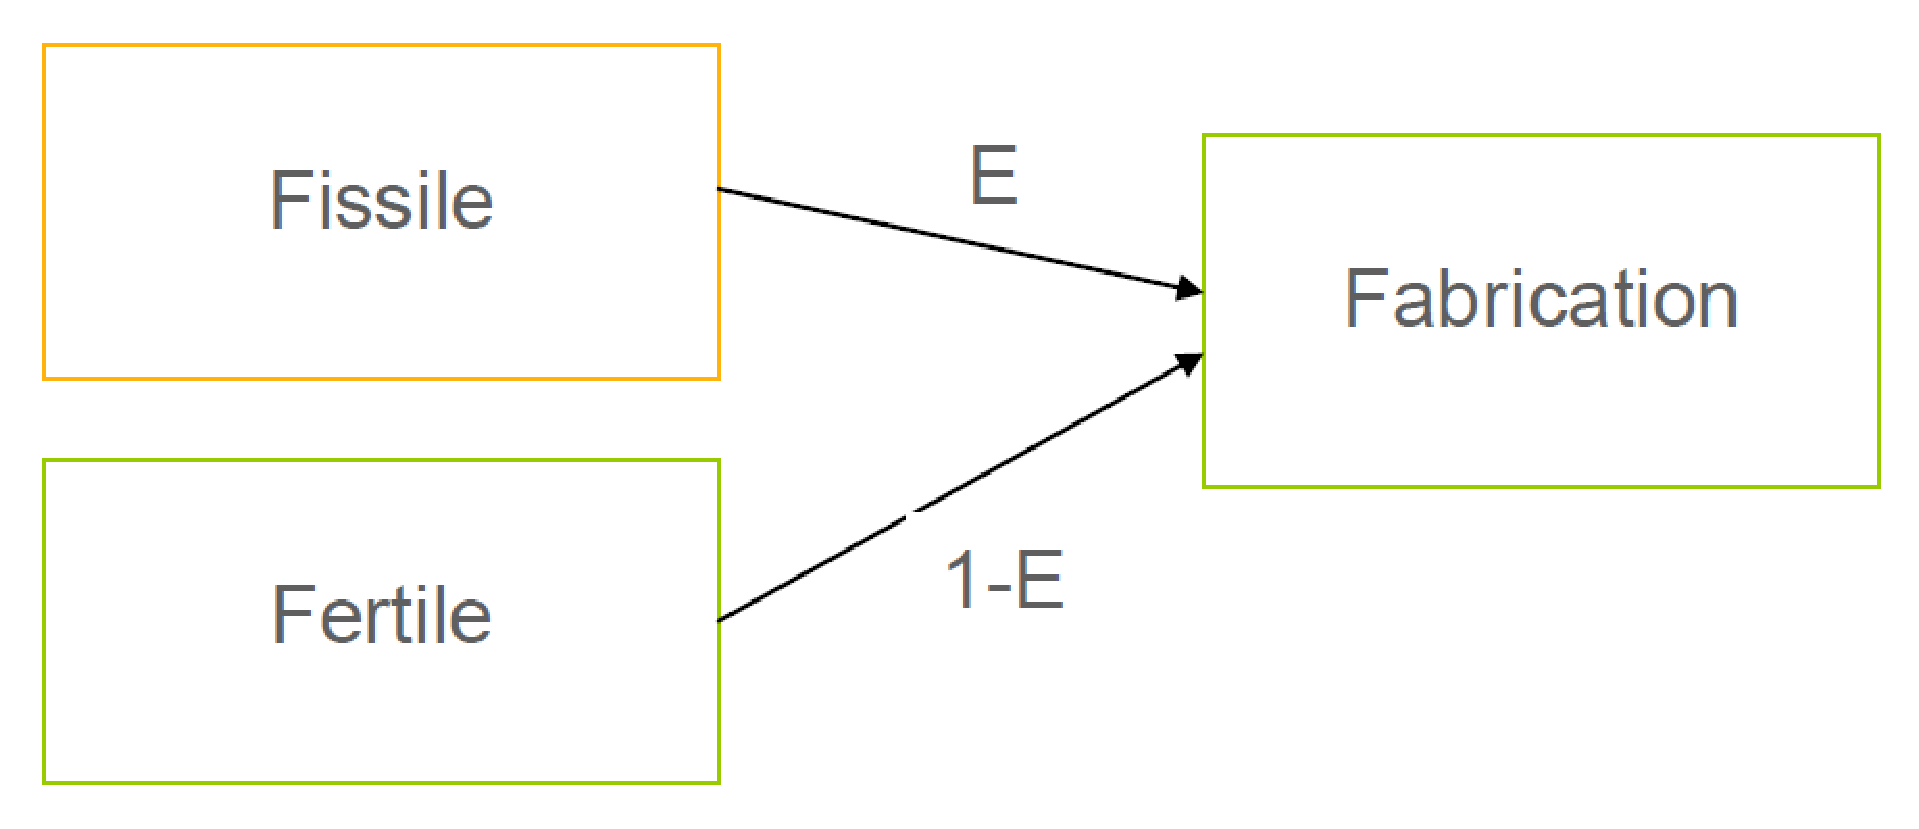
\includegraphics[height=3cm]{./images/equiv.eps}
    \caption{Result of COSI's Equivalence Method. \cite{meyer_new_2009}.}
  \end{figure}
\end{frame}
  
\begin{frame}[ctb!]
  \frametitle{Two Motivating Questions}

  \begin{block}{Dynamic Resource Exchange}
    If facilities are treated as individual black boxes and connections between
    facilities are determined dynamically, how does one match suppliers with
    demanders considering supply constraints and, supply response to
    quality-based demands, and issues of fungibility?
  \end{block}

  \pause

  \begin{block}{Fuel Order Approximation}
    Can one model the interface between separations and recycled fuel
    fabrication more realistically?
  \end{block}

\end{frame}
